\documentclass{beamer}
\usepackage[utf8]{inputenc}
\usepackage[ngerman]{babel}
\usepackage{url}
\usepackage{xcolor}

\usetheme[compress]{Berlin}
\setbeamerfont{headline}{size=\large}
\setbeamerfont*{section in head/foot}{size=\tiny}
\setbeamertemplate{toc}{circle}
\setbeamertemplate{itemize subitem}[triangle] % if you want a triangle
\setbeamercovered{transparent}

\definecolor{myBlue}{rgb}{0,0.55,0.8}
\usecolortheme[named=myBlue]{structure}

\title{Das \LaTeX-KBS}
\subtitle{\small Grundlagen von \LaTeX, Ti\textit{k}Z und Co.}
\author
{
	Walter Stieben \texttt{\href{mailto:4stieben@informatik.uni-hamburg.de}{4stieben@inf}}\\
	\href{http://hauke-stieler.de/}{Hauke Stieler} \texttt{\href{mailto:4stieler@informatik.uni-hamburg.de}{4stieler@inf}}
}
\date{\footnotesize 12.01.2016}

\begin{document}
	\maketitle
	\begin{frame}
		\begin{minipage}[t][0.5\textheight]{0.5\textwidth}
			\vspace{0pt} 
			\tableofcontents
		\end{minipage}
		\begin{minipage}[t]{0.45\textwidth} 
			\vspace{0pt}  
			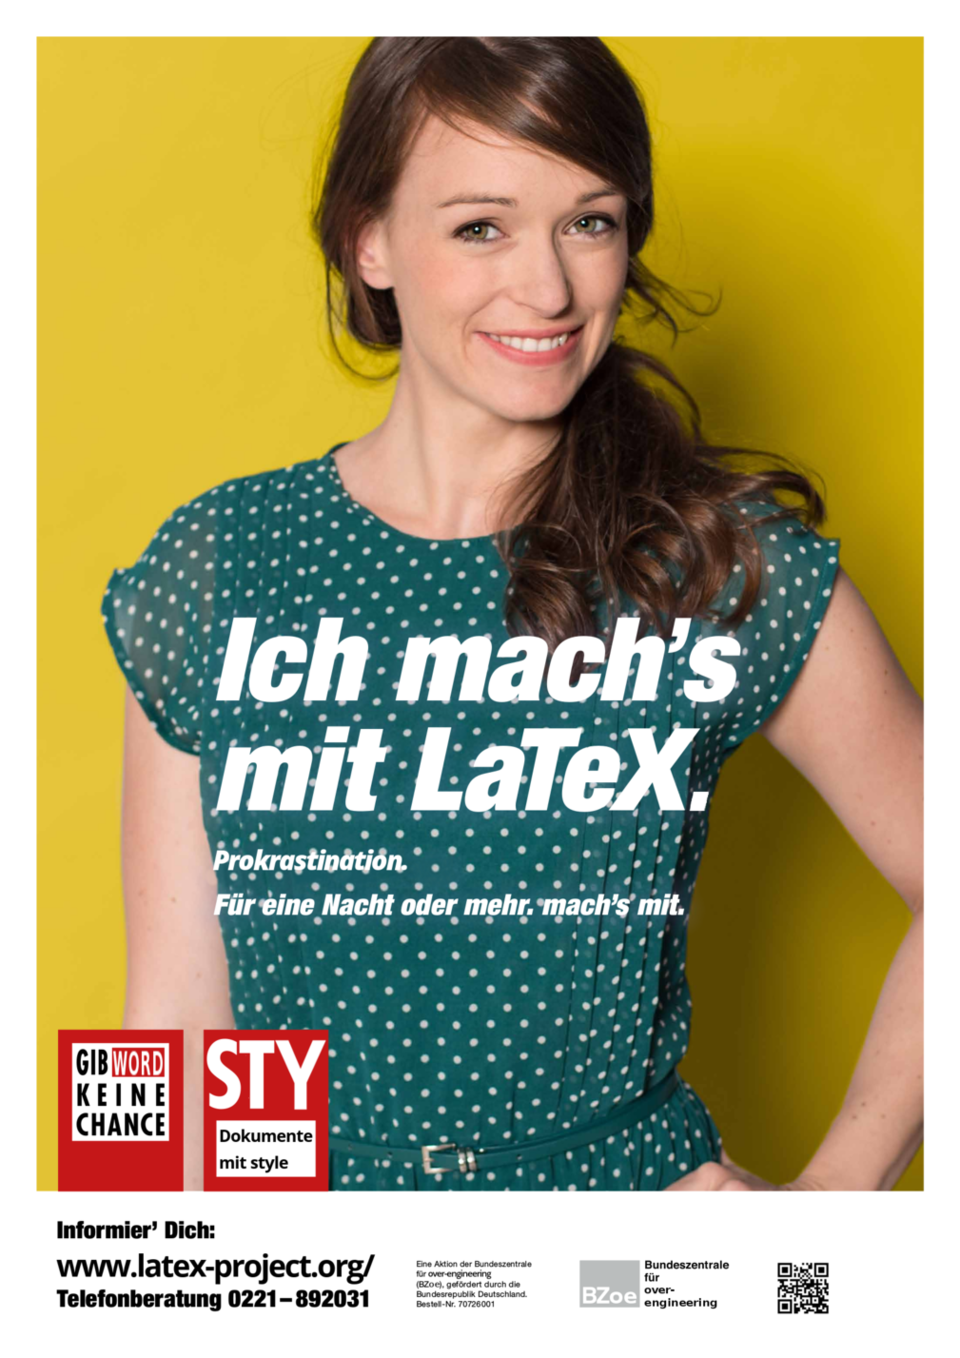
\includegraphics[width=\textwidth]{./images/gib-word-keine-chance}
		\end{minipage}
	\end{frame}
	\section{Was ist \TeX{} und \LaTeX{}}
		\subsection*{asd}
		\begin{frame}{Was ist \LaTeX{}}
			\textbf{\LaTeX{} und \TeX{}:}
			\begin{itemize}
				\item \TeX{} ist ein Textsatzsystem von Donald E. Knuth
				\item \LaTeX{} ist ein Satz von Makros für \TeX
				\item WYSIWYT (What You See Is What You Type)
			\end{itemize}
			\vspace{0.2cm}
			\textbf{Vorteile von \LaTeX{}:}
			\begin{itemize}
				\item Ergebnis sieht hübsch aus
				\item \LaTeX{} kümmert sich um die Formatierung
				\item Der Quelltext lässt sich Versionsverwalten
				\item Für mathematische Formeln sehr gut
				\item ``Ich möchte X mit \LaTeX{} machen'' $\rightarrow$
				Suchmaschine: ``latex X'' eingeben $\rightarrow$
				Ergebnis in den Quelltext kopieren
			\end{itemize}
		\end{frame}
\end{document}